\noindent Here we discuss what happens when Goldstone's theorem related to spontaneous symmetry breaking (SSB) and local gauge invariance are combined. \\

\noindent Consider an $SU(2)$ gauge theory

\begin{equation}
\mathcal{L} = \bar{\psi} ( i \slashed{D} - m) \psi - \frac{1}{4} F_{\mu\nu} F^{\mu\nu}
\end{equation}

\noindent Where the second term represents the auxiliary gauge boson fields that are needed to induce the theory with local gauge invariance. \\

\noindent These (massive) gauge bosons are observed in experiment, and we are inclined to add a bosonic mass term to this theory. Naively, we can add a term of the form $\frac{1}{2} m^2 A_\mu^j (x) A_\mu^j (x)$. Unfortunately, this will break local gauge invariance since it does not obey the local gauge transformation like the gauge boson fields do, e.g., as $A_\mu^j (x) \rightarrow A_\mu^j (x) - \frac{1}{e} \partial_\mu \alpha (x)$. \\

\noindent The local gauge transformation is a \textit{constraint}, and constraints in physics can be solved by adding new degrees of freedom. For example, if we have $N$ equations (constraints) and $M$ unknowns (degrees of freedom), but $N >> M$, then there are no solutions! Therefore, we introduce new degrees of freedom until we get solutions, and, in the context of high energy physics, new degrees of freedoms are fields/particles/excitations! \\

\subsection*{Abelian case}

\noindent We consider the abelian case for the $SU(2)$ gauge theory combined with SSB as the ``toy'' model for such a theory. Consider a theory of a complex scalar field $\phi = \phi_R + i \phi_I$ (which can also be regarded as a doublet) coupled to a $U(1)$ gauge field $A_\mu$

\begin{equation}
\mathcal{L} = |D_\mu \phi |^2 - \frac{1}{4} F_{\mu\nu} F^{\mu\nu} - V(\phi)
\end{equation}

\noindent Where we have the covariant derivative $D_\mu = \partial_\mu + i e A_\mu$ obeying the local gauge condition. \\

\noindent We establish that $\mathcal{L}$ is indeed a gauge theory, since it is invariant under the local gauge transformation, since each term built from the invariant fields are invariant under local gauge transformation. The involved locally gauge invariant fields are

\begin{align}
A_\mu (x) &\rightarrow A_\mu(x) - \frac{1}{e} \partial_\mu \alpha (x) \\
\phi (x) &\rightarrow e^{i \alpha (x)} \phi (x).
\end{align}

\noindent For the interacting part of the theory, consider the potential

\begin{equation}
V(\phi) = -\mu^2 \phi^* \phi + \frac{\lambda}{2} (\phi^* \phi)^2 \text{, } \mu^2 > 0.
\end{equation}

\noindent Note that this potential is quartic in $\phi$, leaving no hope for solving this model straight away. To find a solution, we follow the same steps as for SSB: (1) Find a field value $\phi = \phi_0$ that minimizes the potential $V(\phi)$, and (2) expand the Lagrangian density around the minima and study small fluctuations in the field. \\

\noindent Following the same procedure as before, minimize $V(\phi)$ and we find the family of minima at (\textbf{Exercise}) $\phi_0 = e^{i \varphi} \sqrt{\frac{\mu^2}{\lambda}}$, and choose the $\varphi=0$ point, such that our minima occurs at 

\begin{equation}
\phi_0 = \sqrt{\frac{\mu^2}{\lambda}}.
\end{equation} 

\noindent To study small fluctuations about the minima, write the field as 

\begin{equation}
\phi (x) = \phi_0 + \frac{1}{\sqrt{2}} (\phi_1 (x) + i \phi_2 (x))
\end{equation}

\noindent Where $\phi_1$ and $\phi_2$ are small. Substituting into the potential, it becomes (\textbf{Exercise})

\begin{equation}
V(\phi) = -\frac{\mu^4}{2\lambda} + \mu^2 \phi_1^2 + \dots + \mathcal{O}(\phi_j^3)
\end{equation}

\noindent Where the $\dots$ account for all of the other terms form substituting $\phi(x)$, including $\phi_2$ terms and cross-terms of $\phi_1$ and $\phi_2$. Now expand $\mathcal{L}$ around the minima $\phi_0$ to get

\begin{equation}
\mathcal{L} = \frac{1}{2} |\partial_\mu \phi_1|^2 + \frac{1}{2} |\partial_\mu \phi_2|^2 - \mu^2 \phi_1^2 + \dots + \mathcal{O}(\phi_j^3).
\end{equation}

\noindent Note that other terms exist here, such as cross-terms, indicated by $\dots$, and that we alos have shifted away the constant terms in $\mathcal{L}$. The first two terms are effectively massless, while the third term is effectively massive, since it contains $\mu^2$. Other terms from the covariant derivative term include

\begin{equation}
|D_\mu \phi|^2 =  \frac{1}{2} |\partial_\mu \phi_1|^2 + \frac{1}{2} |\partial_\mu \phi_2|^2 + \sqrt{2} e \phi_0 A_\mu \partial^\mu \phi_2 + e^2 \phi_0^2 A_\mu A^\mu + \dots.
\end{equation}

\noindent We interpret the last term above as the \textit{bosonic mass term}

\begin{equation}
\Delta{\mathcal{L}} = e^2 \phi_0^2 A_\mu A^\mu \equiv \frac{1}{2} m_A^2 A_\mu A^\mu.
\end{equation}

\noindent This result is in the classical, low-energy limit, since we studied only small fluctuations of the field. \\

\noindent To outline the quantization of this theory, we use the path integral approach, although lattice quantization also works for this theory. So, break the Lagrangian density into free and interacting parts $\mathcal{L} = \mathcal{L}_0 + \mathcal{L}_{\text{int}}$, where

\begin{equation}
\mathcal{L}_0 = \frac{1}{2} |\partial_\mu \phi_1|^2 + \frac{1}{2} |\partial_\mu \phi_2|^2 - \mu^2 \phi_1^2 - \frac{1}{4} F_{\mu\nu} F^{\mu\nu}
\end{equation}

\noindent And $\mathcal{L}_{\text{int}}$ is the rest of the terms: perturbations leading to vertices in the Feynman rules. For example, in momentum space, one of the vertices looks like


\begin{figure}[H]\centering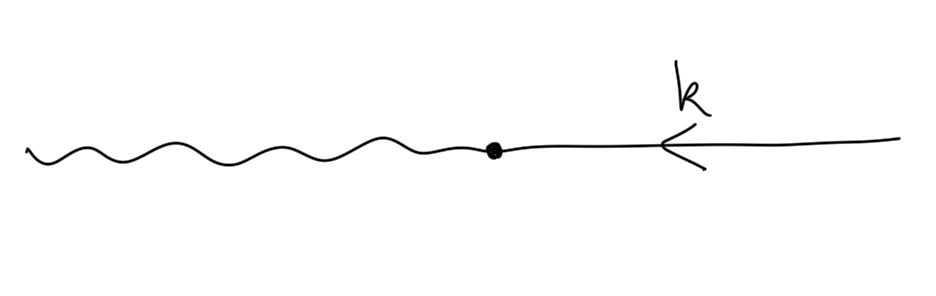
\includegraphics[width=2in]{images/ex_vertex.png} \end{figure} 
\begin{equation} = \sqrt{2} i e \phi_0 (-i k^\mu) \equiv m_A k^\mu \end{equation}

\noindent At the quantum level, the mass of the gauge boson fields manifest in the poles of the Green's functions. For example,


\begin{figure}[H]
	\centering
	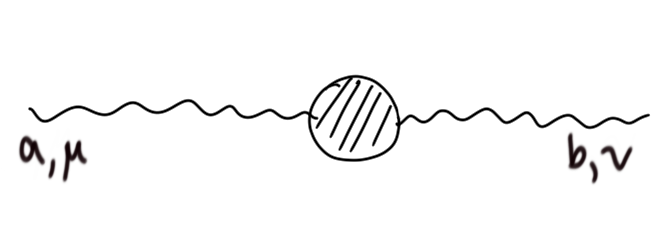
\includegraphics[width=2in]{images/gauge_boson_poles.png}
\end{figure} 
$$\sim$$
\begin{figure}[H]
	\centering
	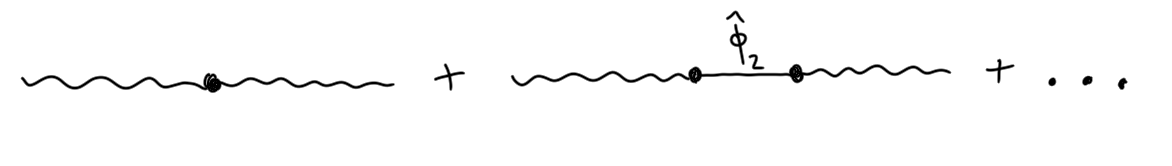
\includegraphics[width=3in]{images/gauge_boson_vertices.png}\end{figure} 
 \begin{equation} 
 = i m_A^2 g^{\mu\nu} + (m_A k^\mu) \frac{i}{k^2} (m_A k^\nu) \sim i m_A^2 
 \end{equation}
 
 \subsection*{Nonabelian case}
 
 \noindent For the nonabelian case of SSB in $SU(2)$ gauge theory, consider a general, continuous gauge group $\mathcal{G}$ and a set of scalar fields $\underline{\phi} = (\phi_1, \phi_2, \dots)$ that transform under $\mathcal{G}$ as
 
 \begin{equation}
 \phi_j \rightarrow (\mathbb{I} + i \alpha^a t^a )_{jk} \phi_k
 \end{equation}
 
 \noindent Where $\alpha$ is small, such that we have the representation of an element $g \in \mathcal{G}$
 
 \begin{equation}
 \pi (g) = e^{i \alpha^a t^a}
 \end{equation}
 
 \noindent And the $\{t^a\}$ are purely imaginary matrices from the associated Lie algebra that depend on the representation. \\
 
 \noindent Now build a gauge theory based on the gauge group $\mathcal{G}$ by promoting it to a local symmetry that acts locally on the scalar fields as
 
 \begin{equation}
 \underline{\phi} (x) \rightarrow \pi (g(x)) \underline{\phi} (x).
 \end{equation}
 
 \noindent Derivatives of the scalar fields in this gauge theory will be the covariant derivative
 
 \begin{equation}
 D_\mu \underline{\phi} = (\partial_\mu + g A_\mu^a T^a ) \underline{\phi}
 \end{equation}
 
 \noindent Where the matrix $T^a = i t^a$. Build the kinetic energy terms by squaring and halving the covariant derivative acting on the field to obtain
 
 \begin{equation}
 \frac{1}{2} (\partial_\mu \phi_j )^2 + g A_\mu^a ( \partial_\mu \phi_j T_{jk}^a \phi_k ) + \frac{1}{2} g^2 A_\mu^a A^{b \mu} (T^a \phi)_j (T^b \phi)_j
 \end{equation}

\noindent Now introduce the aspect of SSB to this gauge theory by combining this with the wine bottle potential

\begin{equation}
V(\underline{\phi}) = -\nu | \underline{\phi} |^2 + \lambda | \underline{\phi} |^4.
\end{equation}

\noindent So, there is a classical minima of these fields at $\underline{\phi}_0$, such that $\underline{\phi} (x) = \underline{\phi}_0 + \epsilon \underline{\phi}_1 (x)$, where $\underline{\phi}_1 (x)$ are small fluctuations about the minima, which we substitute and expand about in the Lagrangian density to find terms like (\textbf{Exercise})

\begin{equation}
\Delta \mathcal{L} \sim \frac{1}{2} (m^2)_{ab} A_\mu^a A^{b \mu}
\end{equation}

\noindent Where we have a negative of a positive semidefinite matrix (if diagonable, then eigenvalues are $\ge 0$) with indices running from $a, \, b = 1, \dots, \text{dim}(\mathcal{G})$

\begin{equation}
(m^2)_{ab} \equiv g^2 (T^a \underline{\phi}_0 )_j (T^b \underline{\phi}_0)_j.
\end{equation}

\noindent For $\mathcal{G} = SU(2)$, choose the fundamental representation in terms of the Pauli spin matrices

\begin{equation}
T^1 = i \sigma^x, \,\,\,\,\,\,\,\, T^2 = i \sigma^y , \,\,\,\,\,\,\,\, T^3 = i \sigma^z.
\end{equation}

\noindent Then the fields (eigenvectors) in this basis are

\begin{equation}
\underline{\phi} = \begin{pmatrix} \phi_1 \\ \phi_2 \end{pmatrix} \text{ and } \underline{\phi}_0 = \begin{pmatrix} 1 \\ 0 \end{pmatrix}.
\end{equation}

\noindent The action of the generators $T^a$ on the minima, the vacuum state, are (\textbf{Exercise})

\begin{align}
T^1 \underline{\phi}_0 &= i \begin{pmatrix} 0 \\ 1 \end{pmatrix} \\
T^2 \underline{\phi}_0 &= - \begin{pmatrix} 0 \\ 1 \end{pmatrix} \\
T^3 \underline{\phi}_0 &= i \begin{pmatrix} 1 \\ 0 \end{pmatrix} 
\end{align}

\noindent Giving matrix elements

\begin{equation}
[m^2] = 
\begin{bmatrix}
 -1 & -i & 0 \\
 -i & -1 & 0 \\
  0 & 0 & -1
\end{bmatrix}.
\end{equation}

\noindent If the generator $T^a$ leaves the vacuum state invariant such that

\begin{equation}
T^a \underline{\phi}_0 = 0
\end{equation}

\noindent Then we get massless bosons!